
\documentclass[calculator,steamtables,refrigeranttables,psychrometricchart,datasheet,solutions]{exam}
%\documentclass[calculator,steamtables,refrigeranttables,psychrometricchart,datasheet]{exam}

% The full list of class options are
% calculator : Allows approved calculator use.
% datasheet : Adds a note that data sheet are attached to the exam.
% handbook : Allows the use of the engineering handbook.
% resit : Adds the resit markings to the paper.
% sample : Adds conspicuous SAMPLE markings to the paper
% solutions : Uses the contents of \solution commands (and \solmarks) to generate a solution file

\usepackage{pdfpages}
\usepackage{lscape,comment}

\coursecode{EG3521}%%
\coursetitle{Engineering Thermodynamics}%
%\coursecode{EG3539}% 
%\coursetitle{Thermodynamics}%

\examtime{00.00--00.00}%
\examdate{00}{05}{2015}%
\examformat{Candidates must attempt \textit{all} questions.}

\newcommand{\frc}{\displaystyle\frac}
\newcommand{\br}[1]{\!\left( #1 \right)}
\newcommand{\abs}[1]{\left| #1 \right|}
\newcommand{\fracd}[2]{\frac{\mathrm{d} #1}{\mathrm{d} #2}}
\newcommand{\fracp}[2]{\frac{\partial #1}{\partial #2}}
\renewcommand{\d}[1]{\mathrm{d} #1 }
\newcommand{\Ma}{\mathrm{M\!a}}



\begin{document}

%%%
%%% QUESTION 1
%%%
\begin{question}

\begin{enumerate}[(a)]

%%%  Q(1.i) Diesel: Example 13.22 (Rajput)
\item The volume ratios of compression and expansion for a diesel engine are 15.3 and 7.5, respectively. The pressure and temperature at the beginning of the compression are 1 bar and 27$^{\text{ o}}$C. Assume that the volume at the end of the isentropic compression is 1 m$^{3}$, determine:
\begin{enumerate}[(i)]
 \item Mean effective pressure $\left(\text{MEP}=\frc{\text{W}_{\text{net}}}{\text{V}_{\text{max}}-\text{V}_{\text{min}}}\right)$;~\marks{7}
%
\solution{ The problem gives: 
     \begin{center}
      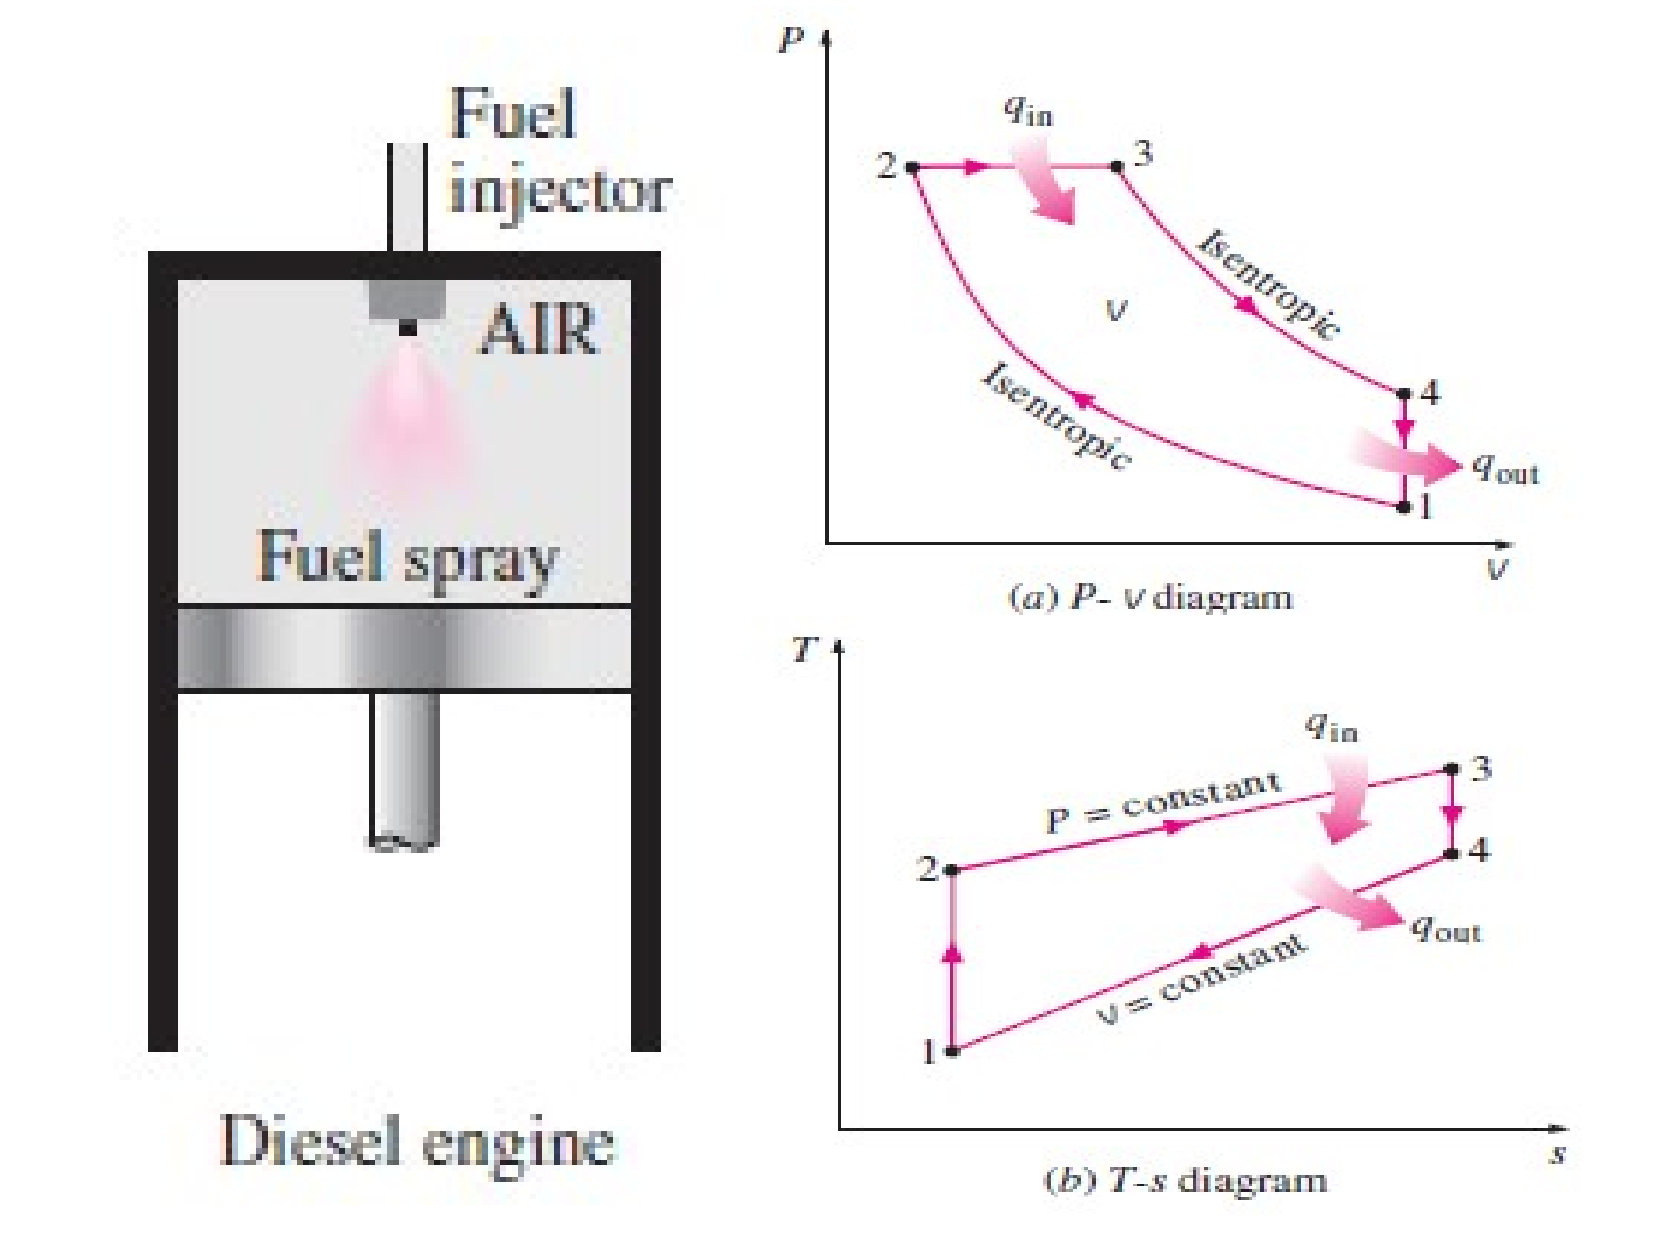
\includegraphics[width=6.cm,clip]{../Thermodynamics/EngThermod/2014-15/Lectures/Pics/InternalCombustion_IdealDieselCycle}
     \end{center} 
\begin{itemize}
 \item $\frc{V_{1}}{V_{2}}$ = 15.3 = r, $\frc{V_{4}}{V_{3}}$ = 7.5;
 \item $P_{1}$ = 1 bar; $T_{1}$ = 27$^{\circ}$C = 300.15 K; V$_{2}$ = 1 m$^{3}$
\end{itemize}


The first step to solve the problem is to calculate T$_{2}$, P$_{2}$, T$_{3}$, T$_{4}$ and P$_{4}$:
\begin{description}
\item[1-2:] adiabatic compression:  ~\solmarks{1/7} 
\begin{eqnarray}
&& T_{1}V_{1}^{\gamma-1}=T_{2}V_{2}^{\gamma-1} \rightarrow T_{2} = 893.75\; \text{K} \nonumber  \\
&& P_{1}V_{1}^{\gamma}=P_{2}V_{2}^{\gamma} \rightarrow P_{2} = 45.56\; \text{bar}  \nonumber
\end{eqnarray}

\item[2-3:] heat addition at constant pressure: ~\solmarks{0.5/7}
\begin{displaymath}
\frc{V_{2}}{T_{2}} = \frc{V_{3}}{T_{3}} \rightarrow T_{3} = T_{2}\frc{V_{3}}{V_{1}}\frc{V_{1}}{V_{2}} = 1823.25\text{ K }
\end{displaymath}

\item[3-4:] adiabatic expansion:~\solmarks{1/7} 
\begin{eqnarray}
&& T_{3}V_{3}^{\gamma-1}=T_{4}V_{4}^{\gamma-1} \rightarrow T_{4} = 814.37\; \text{K} \nonumber  \\
&& P_{3}V_{3}^{\gamma}=P_{4}V_{4}^{\gamma} \rightarrow P_{4} = 2.71\; \text{bar}  \nonumber
\end{eqnarray}
\end{description}

Now calculating MEP:~\solmarks{1.5/7}
\begin{displaymath}
MEP = \frc{W_{\text{net}}}{V_{\text{max}}-V_{\text{min}}} = \frc{m\left[C_{p}\left(T_{3}-T_{2}\right) - C_{v}\left(T_{4}-T_{1}\right)\right]}{V_{1}-V_{2}}
\end{displaymath}
 now we need to calculate the mass (m) via the equation of state of ideal gas at state 2:~\solmarks{1/7}
\begin{displaymath}
m = \frc{P_{2}V_{2}}{R T_{2}} MW = 17780.98 g \approx 17.78\; kg
\end{displaymath}
with the mass of air, the MEP is 7.02 bar~\solmarks{2/7}
}
%
 \item Cycle efficiency $\left(\eta_{\text{Diesel}}=\frc{\text{W}_{\text{net}}}{\text{Heat Supplied}}\right)$.~\marks{3}
\solution{The efficiency of the Diesel engine is given by:~\solmarks{3/3}
\begin{displaymath}
\eta_{\text{Diesel}} = \frc{W_{\text{net}}}{\text{Heat Supplied}} = \frc{m\left[C_{p}\left(T_{3}-T_{2}\right) - C_{v}\left(T_{4}-T_{1}\right)\right]}{m C_{p}\left(T_{3}-T_{2}\right)} = 0.6048
\end{displaymath}
}
%
\end{enumerate}

%%% Q(1.ii) Brayton: Example 10.1 (Borgnakke )
\item In an ideal air-standard Brayton cycle, air enters the compressor at 0.1 MPa and 15$^{\circ}$C and leaves at 1 MPa. The maximum temperature of the cycle is 1100$^{\circ}$C:
\begin{enumerate}[(i)]
\item Sketch $Pv$ (pressure $\times$ specific volume) and $Ts$ (temperature $\times$ specific entropy) diagrams for the cycle, numbering each stage;~\marks{2}
\solution{ Schematics, $Pv$ and $Ts$ diagrams:\solmarks{2/2}
   \begin{center}%
     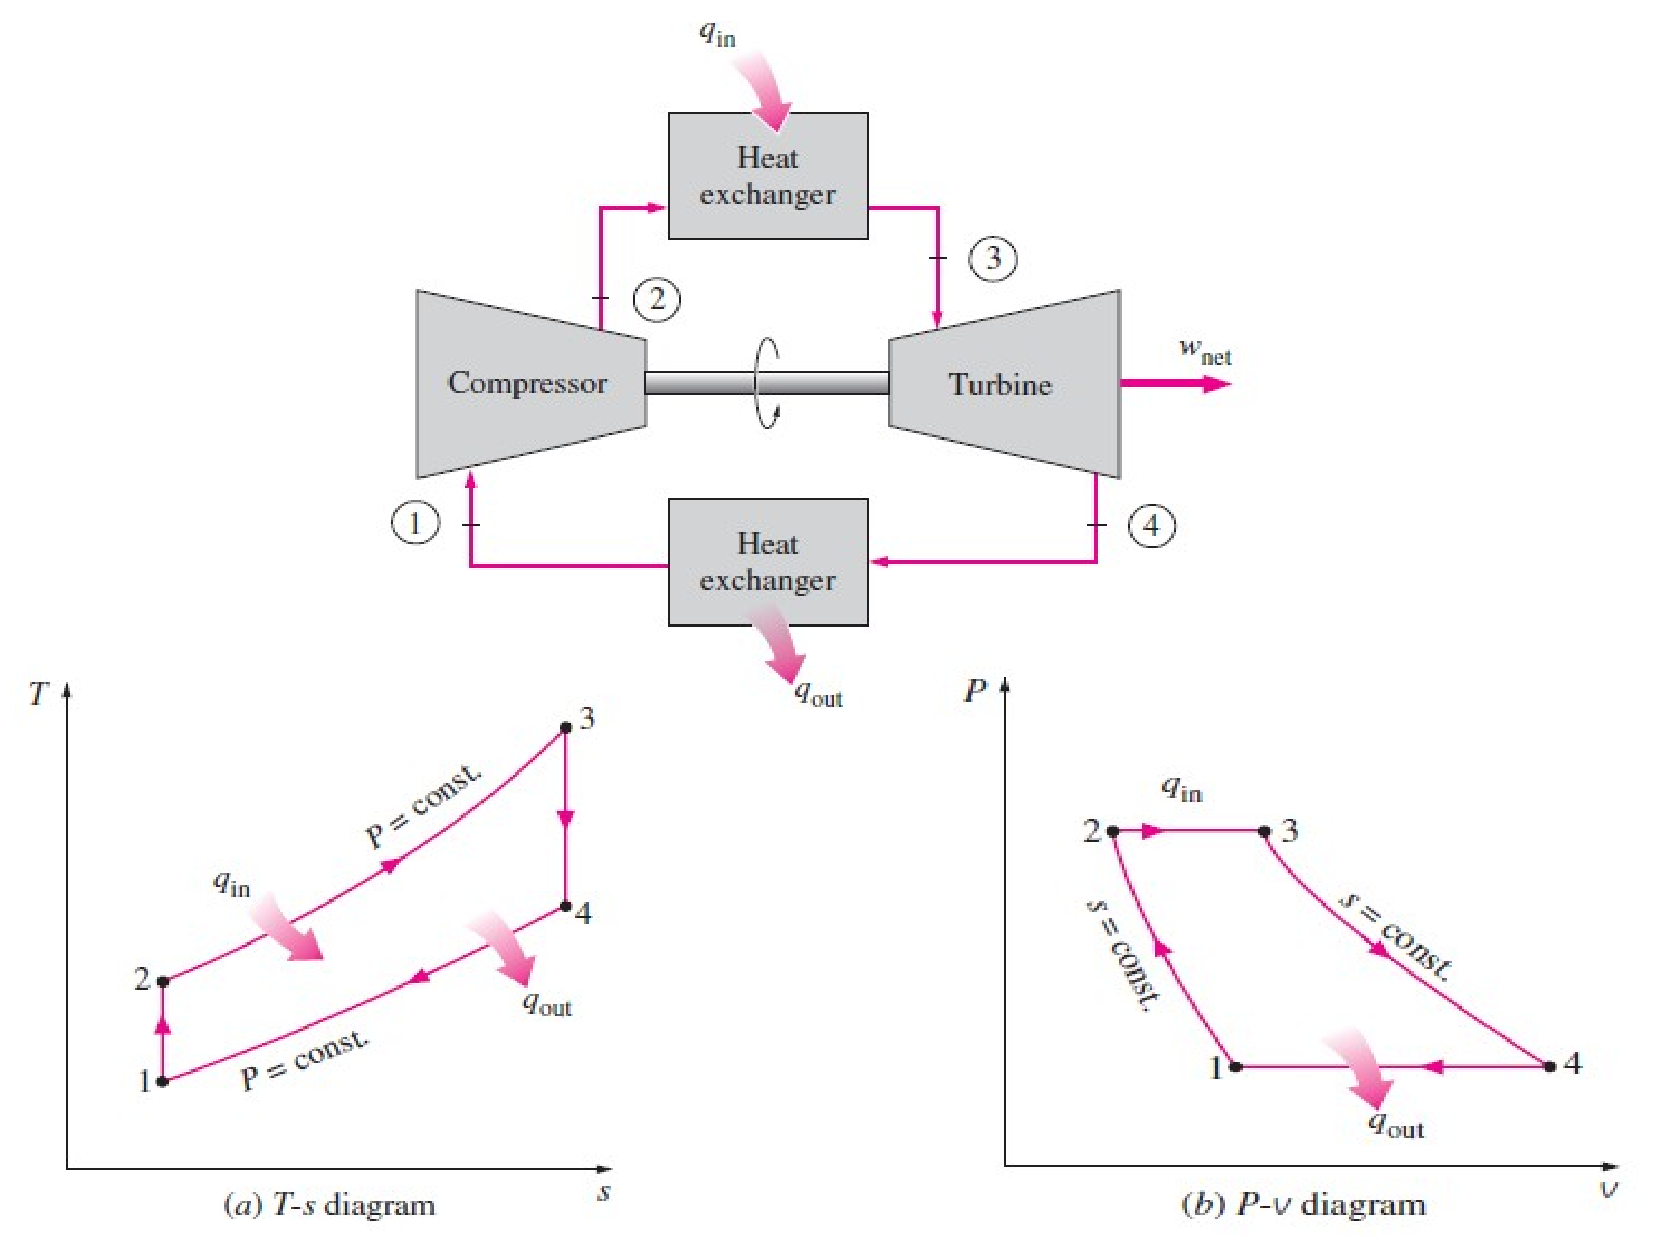
\includegraphics[height=8.cm,width=8.5cm,clip]{../Thermodynamics/EngThermod/2014-15/Lectures/Pics/Brayton_cycle1}
   \end{center}  
}
%
\item Calculate the temperature of the fluid leaving the compressor and the turbine;~\marks{2}
\solution{ Calculating T$_{2}$ and T$_{4}$:
\begin{description}
\item[1-2:] isentropic compression: \solmarks{1/2}
\begin{displaymath}
T_{1}P_{1}^{\frac{1-\gamma}{\gamma}} = T_{2}P_{2}^{\frac{1-\gamma}{\gamma}} \rightarrow T_{2} = 556.33\text{ K}
\end{displaymath}
\item[3-4:] isentropic expansion: \solmarks{1/2}
\begin{displaymath}
T_{3}P_{3}^{\frac{1-\gamma}{\gamma}} = T_{4}P_{4}^{\frac{1-\gamma}{\gamma}} \rightarrow T_{4} = 711.22 \text{ K}
\end{displaymath}
\end{description}
}
%
\item Determine the efficiency of the cycle $\left(\eta_{\text{Brayton}}=\frc{\text{W}_{\text{net}}}{\text{Heat Supplied}}\right)$;~\marks{2}
\solution{ Work required by the compressor~\solmarks{0.5/2} 
\begin{displaymath}
W_{\text{C}} = h_{2}-h_{1} = C_{p}\left(T_{2}-T_{1}\right) = 269.52 \text{ kJ.kg}^{-1}
\end{displaymath}
And the work produced by the turbine:~\solmarks{0.5/2}
\begin{displaymath}
W_{\text{T}} = h_{4}-h_{3} = C_{p}\left(T_{4}-T_{3}\right) = -665.24 \text{ kJ.kg}^{-1}
\end{displaymath}
The efficiency is given by:~\solmarks{1/2}
\begin{displaymath}
\eta_{\text{Brayton}} = \frc{W_{\text{net}}}{\text{heat supplied}} = \frc{\left|W_{T}+W_{C}\right|}{C_{p}\left(T_{3}-T_{2}\right)} = 0.4821
\end{displaymath}
}
%
\item Now, assuming that the efficiency of the compressor and the turbine are 80$\%$ and 85$\%$, respectively, and the pressure drop between the compressor and the turbine is 15 kPa. Calculate the work in the compressor and turbine, and the efficiency of the cycle.~\marks{4}
\solution{As the cycle is no longer ideal, temperature after the turbine calculated in (b) is T$_{2s}$ (i.e., calculated from isentropic compression) and actual T$_{2}$ can be recalculated as~\solmarks{1/4}
\begin{displaymath}
\eta_{c}^{\text{(actual)}} = \frc{h_{2s}-h_{1}}{h_{2}-h_{1}} = \frc{T_{2s}-T_{1}}{T_{2}-T_{1}}=0.80\;\rightarrow T_{2}=623.38\text{ K}
\end{displaymath}
And the flow across the turbine,
\begin{displaymath}
\eta_{T}^{\text{(actual)}} = \frc{h_{3}-h_{4}}{h_{3}-h_{4s}} = \frc{T_{3}-T_{4}}{T_{3}-T_{4s}}
\end{displaymath}
However: $\Delta P = P_{2}-P_{3}$ = 15 kPa $\rightarrow P_{3} = 9.85$ bar~\solmarks{0.5/4}. Thus 
\begin{displaymath}
T_{3}P_{3}^{\frac{1-\gamma}{\gamma}} = T_{4s}P_{4}^{\frac{1-\gamma}{\gamma}}\;\rightarrow T_{4s} = 714.30\text{ K}
\end{displaymath}
Now calculating T$_{4}$,~\solmarks{0.5/4}
\begin{displaymath}
\eta_{T}^{\text{(actual)}} = \frc{T_{3}-T_{4}}{T_{3}-T_{4s}} \;\;\rightarrow \;\; T_{4}=813.13\text{ K}
\end{displaymath}
And the power in the turbine and compressor:~\solmarks{1/4}
\begin{eqnarray}
&& W_{C}^{\text{(actual)}} = Cp\left(T_{2}-T_{1}\right) = 336.91 \text{ kJ.kg}^{-1} \nonumber \\
&& W_{T}^{\text{(actual)}} = Cp\left(T_{4}-T_{3}\right) = -562.82 \text{ kJ.kg}^{-1} \nonumber
\end{eqnarray}
And the efficiency:~\solmarks{1/4}
\begin{displaymath}
\eta_{\text{Brayton}}^{\text{(actual)}} = \frc{W_{net}}{Q_{in}} = 0.30
\end{displaymath}

}
%
\end{enumerate}

\end{enumerate}
For this question, assume that air behaves as an ideal gas with the following properties: MW = 29 g.mol$^{-1}$, C$_{p}$ = 1.005 kJ.(kg.K)$^{-1}$ and C$_{v}$ = 0.718 kJ.(kg.K)$^{-1}$, where MW is the molar mass and C$_{p}$ and C$_{v}$ are the heat capacities at constant pressure and volume, respectively. Also, given the following relations for isentropic operations:% with $\gamma = \displaystyle\frac{C_{p}}{C_{v}}$:
\begin{displaymath}
TV^{\gamma-1}=\text{const.} \Leftrightarrow TP^{\frac{1-\gamma}{\gamma}}=\text{const.} \Leftrightarrow PV^{\gamma}=\text{const.} \;\;\;\text{ with } \gamma = \frc{C_{p}}{C_{v}}
\end{displaymath}

\end{question}

\clearpage

%%%
%%% Question 02 
%%%
\begin{question}
%
\begin{enumerate}[(a)]
\item  A geothermal power station (Rankine cycle) uses propane $\left(\text{n-C}_{3}\right)$ as working fluid to produce power $\left(W_{T}\right)$ in a turbine (isentropic expansion) with efficiency $\left(\eta_{T}\right)$ of 90$\%$. Propane is vaporised by geothermal water (i.e., brine, $A-B$ in the diagram) at 90$^{\circ}$C. After condensed, propane is driven to a heat exchanger and the cycle continues. The mass flow rate of propane $\left(\dot{m}_{C3}\right)$ is 250 kg.s$^{-1}$ and the heat capacity at constant pressure $\left(C_{p}\right)$ of brine is 3565.5 J.(kg.K)$^{-1}$. Conditions for propane and brine flows are described in the table below.
%\vspace{-.9cm}
\begin{center}
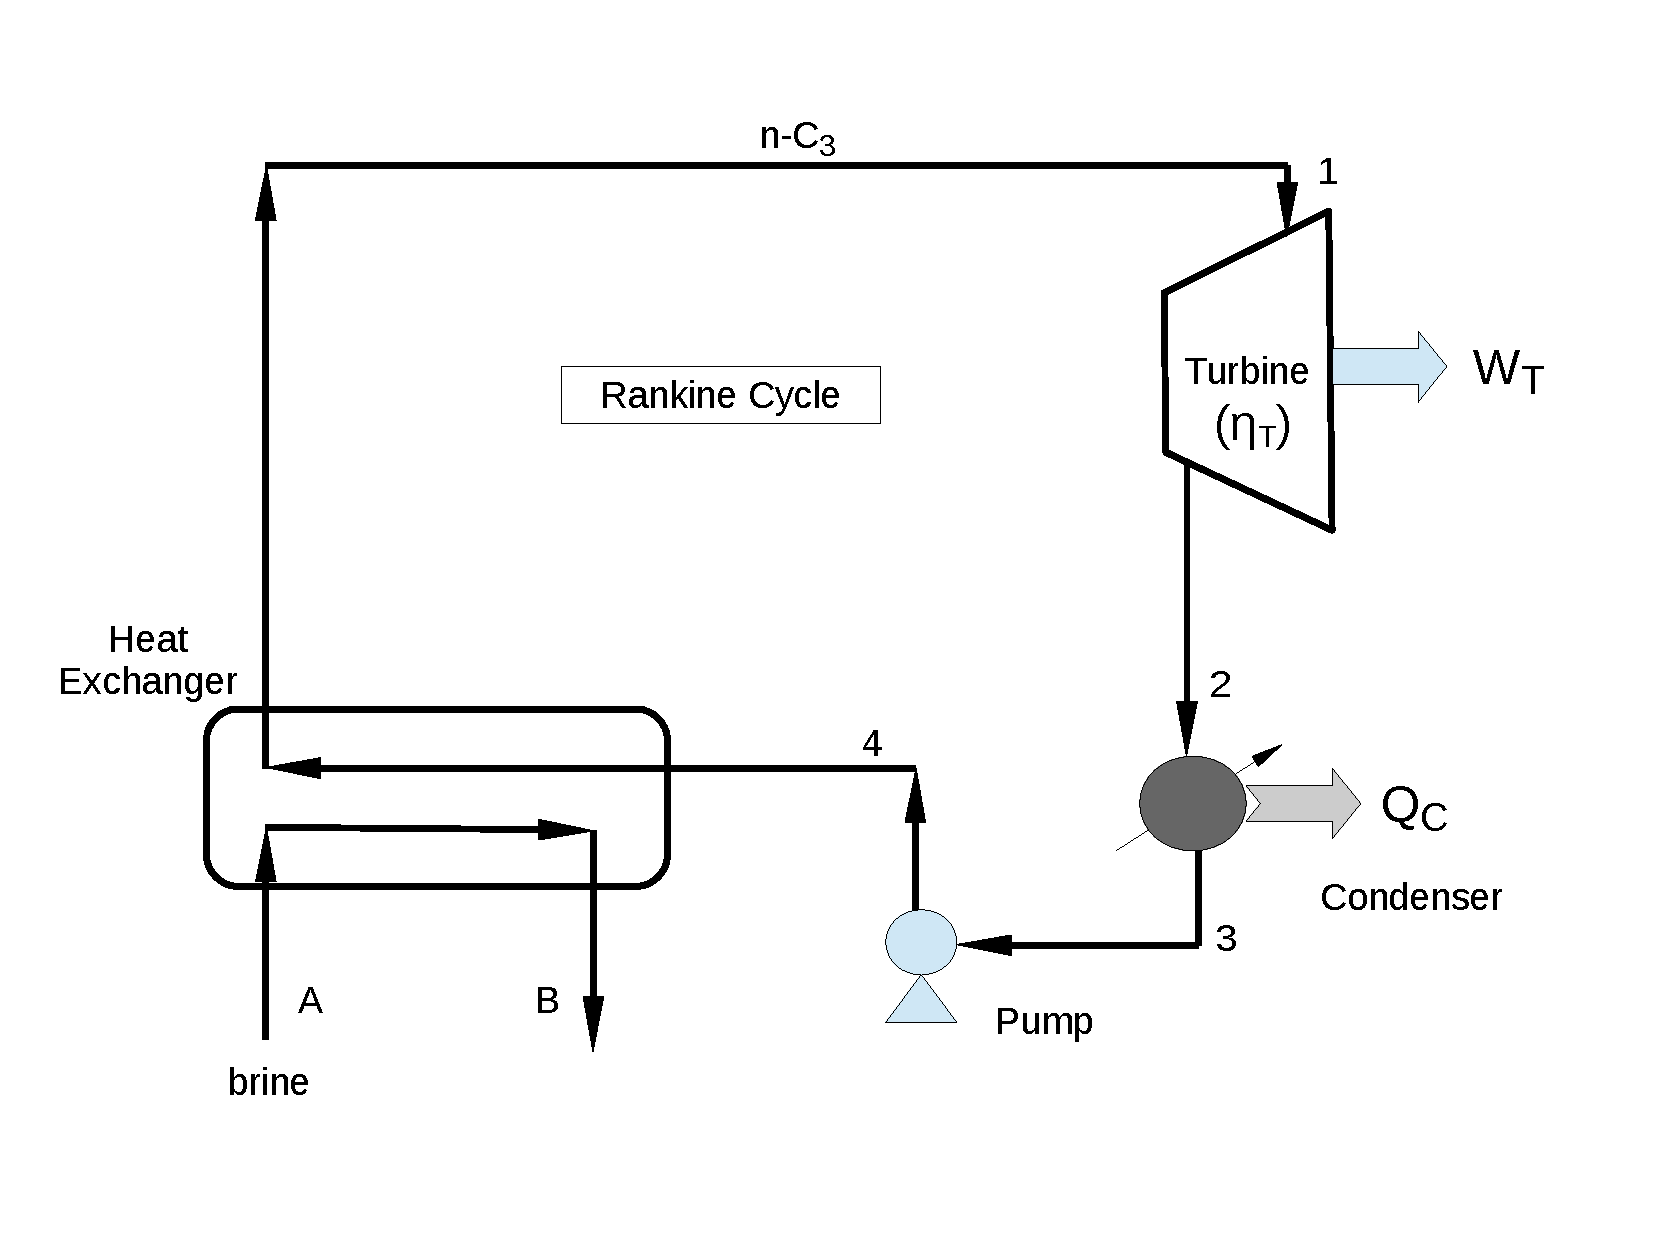
\includegraphics[width=10.cm,height=7.cm,clip]{./Pics/RankineCycle}
%\caption{ Reheat and regenerative Rankine cycle with 2 turbines.}
%\label{exam_mod02_rankinecycle}
\end{center} 
%\vspace{-1.5cm}
\begin{center}
\begin{tabular} {||c | c c c c c c || }
\hline\hline
{\bf Stage} & {\bf P}    & {\bf T}        & {\bf State}    &  {\bf Quality }     &  {\bf h}             & {\bf s}                  \\
            & {\bf (bar)}& {\bf ($^{o}$C)} &               &                     & {\bf (kJ.kg$^{-1}$)}  & {\bf (kJ.(kg.K)$^{-1}$)}  \\
\hline\hline
 {\bf 1 }   & 40         & 100            &   {\bf (a)}    &    --               & {\bf (b)}           & {\bf (c)}                \\
 {\bf 2 }   & 10         &  --            &   --           & {\bf (d)}           & {\bf (e)}           & {\bf (f)}                 \\
 {\bf 3 }   & --         & --             &   {\bf (g)}    & --                  & {\bf (h)}           & {\bf (i)}                \\
 {\bf 4 }   & {\bf (j)}  & --             &   {\bf (k)}    & --                  & {\bf (l)}           & --                      \\
 {\bf A }   & --         & 90             &   --           & --                  & --                  & --                       \\
 {\bf B }   & --         & 30             &   --           & --                  & --                  & --                       \\
 \hline\hline
\end{tabular}
\end{center}

\begin{enumerate}[(i)]
%%
%% Question A
%%
\item In this Table, determine {\it (a)-(l)}.~\marks{6}
%
\solution{
In order to fill the Table we need to calculate the thermodynamic properties for each stage of the cycle:
\begin{description}
%%%
\item[Stage 1:] At P$_{1}$ = 16 bar, T$_{1}$ = 100$^{\circ}$C $>$ T$_{sat}\left(P_{1}\right)$ = 93.38$^{\circ}$C. Therefore the fluid is at {\bf superheated state (SHS)}~\solmarks{0.5/6}. From the superheated table for n-C$_{3}$ at P$_{1}$ and T$_{1}$, we can obtain:\\
{\bf h$_{1}$ = 549.7 kJ.kg$^{-1}$}~\solmarks{0.5/6} and\\
{\bf s$_{1}$ = 1.70 kJ.(kg.K)$^{-1}$}~\solmarks{0.5/6}. 
%%%
\item[Stage 2:] At P$_{2}$ = 10 bar, the fluid is wet vapour after the isentropic expansion. We should first calculate the quality of the vapour in an ideal expansion (using values of entropy/enthalpy obtained from the saturated n-C$_{3}$ table at P$_{2}$.
\begin{displaymath}
x_{2s} =\frc{s_{2s}-s_{f}}{s_{g}-s_{f}} = \frc{1.7 - 0.618}{1.723-0.618} = 0.9792
\end{displaymath}
now to calculate the ideal enthalpy,
\begin{displaymath}
x_{2s} = 0.9792 = \frc{h_{2s}-h_{f}}{h_{g}-h_{f}} = \frc{h_{2s}-166.1}{497.9-166.1}\;\;\Longleftrightarrow\;\; h_{2s} = 491 \frc{kJ}{kg}
\end{displaymath}
As the efficiency of the turbine is of 90$\%$,~\solmarks{0.5/6}
\begin{displaymath}
\eta_{\text{Turbine}} = 0.90 =\frc{h_{2}-h_{1}}{h_{2s}-h_{1}} \;\;\Longleftrightarrow \;\; {\bf h_{2} = 496.87\frc{kJ}{kg}}
\end{displaymath}
Calculating the actual quality using the expressions above, ${\bf x_{2}=0.9969}$~\solmarks{0.5/6} and ${\bf s_{2}=1.7196\text{ kJ.(kg.K)}^{-1}}$.~\solmarks{0.5/6} 
%%%
\item[Stage 3:] At P$_{3}$ = P$_{2}$ = 10 bar, the fluid leaving the condenser towards the pump is {\bf saturated liquid}~\solmarks{0.5/6}, and the enthalpy and specific volume are the same of the liquid phase obtained from the saturated table:\\
{\bf h$_{3}$} = h$_{f}\left(\text{P = 10 bar}\right)$ {\bf = 166.1 kJ.kg$^{-1}$}~\solmarks{0.5/6} \\
{\bf s$_{3}$} = s$_{f}\left(\text{P = 10 bar}\right)$ {\bf = 0.618 kJ.(kg.K)$^{-1}$}~\solmarks{0.5/6} \\
v$_{3}$ = v$_{f}\left(\text{P = 10 bar}\right)$ = 2.043$\times$10$^{-3}$ m$^{3}$.kg$^{-1}$ 
%%%
\item[Stage 4:] The fluid leaving the pump suffered a isentropic compression and we assumed it is incompressible with ${\bf P_{4}=P_{1}=40\text{ bar}}$.~\solmarks{0.5/6} As there is no heat loss in the pump, we can assume $dH \approx VdP$, therefore
\begin{displaymath}
{\bf h_{4}} = h_{3} + v_{3}\left(P_{4}-P_{3}\right) = {\bf= 172.23 \frc{kJ}{kg}}
\end{displaymath}~\solmarks{0.5/6}
As $h_{4} < h_{f,4}\left(P=40\text{ bar}\right)=401 \frc{kJ}{kg}$, the fluid is a {\bf subcooled liquid state (SLS)}.~\solmarks{0.5/6}

\end{description}
Thus the Table becomes:
\begin{center}
\begin{tabular} {||c | c c c c c c || }
\hline\hline
{\bf Stage} & {\bf P}    & {\bf T}        & {\bf State}    &  {\bf Quality }     &  {\bf h}             & {\bf s}                  \\
            & {\bf (bar)}& {\bf ($^{o}$C)} &               &                     & {\bf (kJ.kg$^{-1}$)}  & {\bf (kJ.(kg.K)$^{-1}$)}  \\
\hline\hline
 {\bf 1 }   & 40         & 100            &   {\bf SHS}    &    --               & {\bf 549.7}         & {\bf 1.70}                \\
 {\bf 2 }   & 10         &  --            &   --           & {\bf 0.9969}        & {\bf 496.87}        & {\bf 1.7196}              \\
 {\bf 3 }   & --         & --             &{\bf Sat Liq.}  & --                  & {\bf 166.1}         & {\bf 0.618}                \\
 {\bf 4 }   & {\bf 40}   & --             &   {\bf SLS}    & --                  & {\bf 172.23}        & --                      \\
 {\bf A }   & --         & 90             &   --           & --                  & --                  & --                       \\
 {\bf B }   & --         & 30             &   --           & --                  & --                  & --                       \\
 \hline\hline
\end{tabular}
\end{center}
}
%%
%% Question B
%%
\item Calculate the power produced by the turbine $\left(W_{T}\right)$ and the heat extracted in the condenser $\left(Q_{C}\right)$ in {\it MW}.~\marks{2}
%
\solution{
\begin{displaymath}
{\bf W_{T}} = \dot{m}_{C3} \left(h_{2}-h_{1}\right) = -13207.5 \frc{kJ}{s} {\bf = 13.21 MW}
\end{displaymath}~\solmarks{1/2}

\begin{displaymath}
{\bf Q_{C}} = \dot{m}_{C3} \left(h_{3}-h_{2}\right) = -82692.5 \frc{kJ}{s} {\bf = 82.69 MW}
\end{displaymath}~\solmarks{1/2}
} 
%%
%% Question C
%%
\item Calculate the mass flow rate of brine (A-B) in {\it kg.s}$^{-1}$.~\marks{2}
%
\solution{
The heat extracted by the n-C$_{3}$ $\left(\dot{Q}_{HE,nC3}\right)$ fluid in the heat exchanger can be easily calculated by~\solmarks{1/2}
\begin{displaymath}
{\bf \dot{Q}_{HE,nC3}} = \dot{m}_{C3}\left(h_{1}-h_{4}\right) {\bf = 94367.5\frc{kJ}{s}}
\end{displaymath}
Assuming all heat is transferred from the brine to the propane (i.e., no heat losses to the environment),~\solmarks{1/2} 
\begin{eqnarray}
&& \dot{Q}_{\text{HE,nC3}} + \dot{Q}_{\text{HE,Brine}} = 0 \nonumber \\
&& \dot{Q}_{\text{HE,Brine}} = -94367.5 = \dot{m}_{\text{Brine}} C_{p,\text{Brine}}\left(T_{B}-T_{A}\right) \;\;\rightarrow \;\; {\bf \dot{m}_{\text{Brine}}  = 441.12 \text{ kJ.kg}^{-1}} \nonumber
\end{eqnarray}
}
%%%
%%% Question D
%%%
\item Sketch the $Ts$ (temperature $\times$ specific entropy) diagram for the process indicating the liquid and vapour saturated lines and each stage of the n-C$_{3}$ Rankine cycle.~\marks{3}
%
\solution{~\solmarks{3/3}
\begin{center}
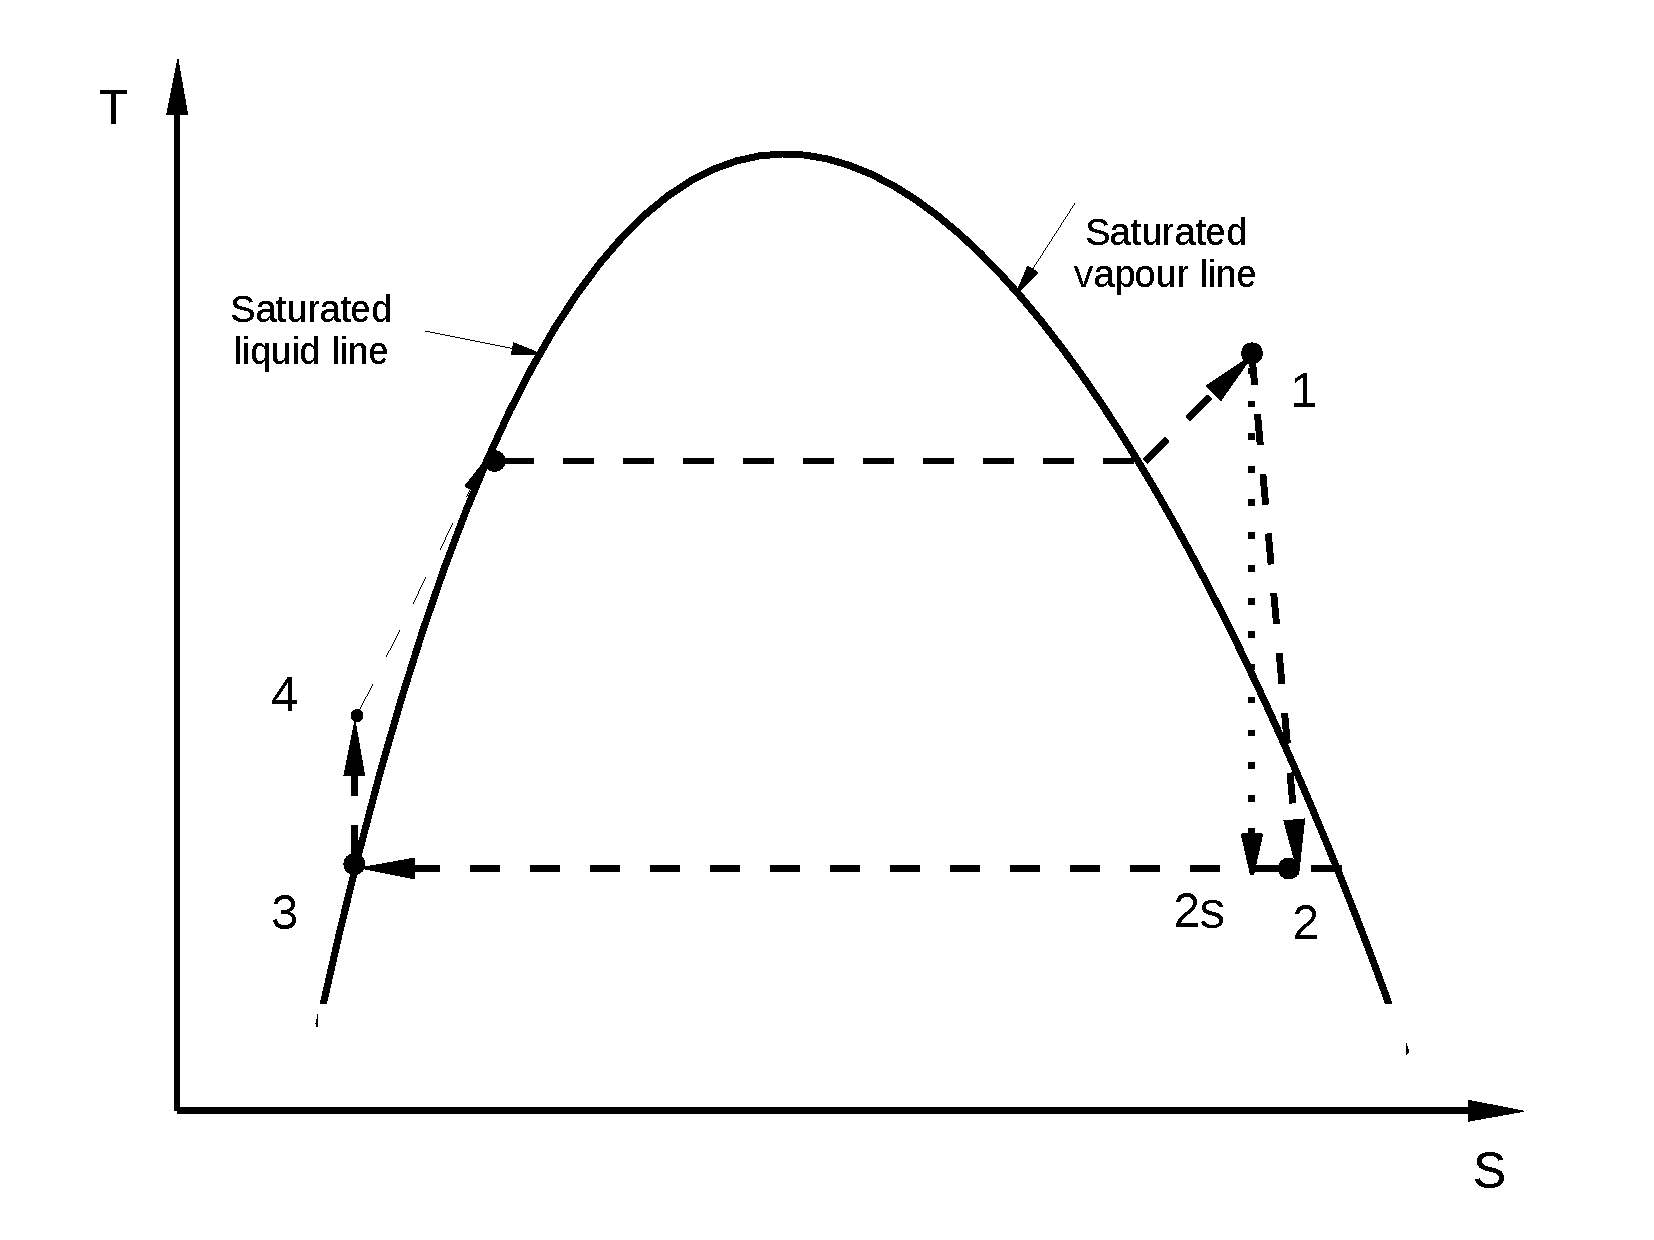
\includegraphics[width=8.cm,clip]{./Pics/TS_DIagramGeothermalBinary2}
\end{center}%~\solmarks{3/3}
}
\end{enumerate} 

To solve this problem, you should assume that the saturated liquid streams are incompressible, and therefore $dh = vdP$ (where $h$, $v$ and $P$ are specific enthalpy, volume and pressure, respectively). Quality of the vapour is expressed as
\begin{displaymath}
x_{j} = \frc{\Psi_{j}-\Psi_{f}}{\Psi_{g}-\Psi_{f}}\;\;\;\text{with }\Psi=\left\{h,s\right\}
\end{displaymath}
where $s$ is the entropy. Efficiency of the turbine $\left(\eta_{\text{Turbine}}\right)$ is given by,
\begin{displaymath}
\eta_{\text{Turbine}} =\frc{h_{2}-h_{1}}{h_{2s}-h_{1}}
\end{displaymath}
where $h_{2s}$ is the enthalpy of stream $2$ assuming ideal turbine performance (i.e., reversible expansion). 



% (Shapiro 2.34) 
\item Air contained in a piston-cylinder system undergoes three consecutive processes,
\begin{itemize} 
\item Process 1--2: Isobaric cooling with P$_{1}$=69 kPa and V$_{1}$=0.11 m$^{3}$;
\item Process 2--3: Isochoric heating with P$_{3}$=345 kPa;
\item Process 3--1: Polytropic expansion, with $PV=$ {\it constant}. %Expansion to the initial state, during which the pressure-volume relationship is $PV=$ {\it constant}.
\end{itemize}  
\begin{enumerate}[(i)]
\item Calculate V$_{2}$ $\left(\text{in m}^{3}\right)$.~\marks{2} 
\solution{
For Process 2--3: V$_{2}$=V$_{3}$. However the expansion 3--1 follows $PV=$ constant,
\begin{displaymath}
P_{1}V_{1}=P_{3}V_{3} \Longrightarrow V_{3} = \frc{P_{1}V_{1}}{P_{3}} = {\bf 0.022\;\text{m}^{3} = V_{2}}
\end{displaymath}~\solmarks{2/2}
}
\item Calculate the work (in $kJ$) for each process.~\marks{3}
\solution{\noindent
Process 1--2: 
\begin{displaymath}
{\bf W_{1-2}} = \int\limits_{V_{1}}^{V_{2}} P dV = P\left(V_{2}-V_{1}\right) = -6072 J \Rightarrow {\bf -6.072 kJ}
\end{displaymath}~\solmarks{1/3}
\noindent
Process 2--3: V$_{2}$=V$_{3}$ $\Longrightarrow$ {\bf W$_{2-3}$ = 0}~\solmarks{1/3} \\
\noindent
Process 3--1: $PV = C$
\begin{displaymath} 
{\bf W_{31}} = \int\limits_{V_{3}}^{V_{1}}P dV = \int\limits_{V_{3}}^{V_{1}}\frc{C}{V} dV = P_{1}V_{1}\ln\frc{V_{1}}{V_{3}} = 12220 J \Rightarrow {\bf 12.22 kJ} 
\end{displaymath}~\solmarks{1/3}
}
\item Sketch the $PV$ (pressure $\times$ volume) diagram for these processes.~\marks{2}
\solution{\solmarks{2/2}
\begin{center}
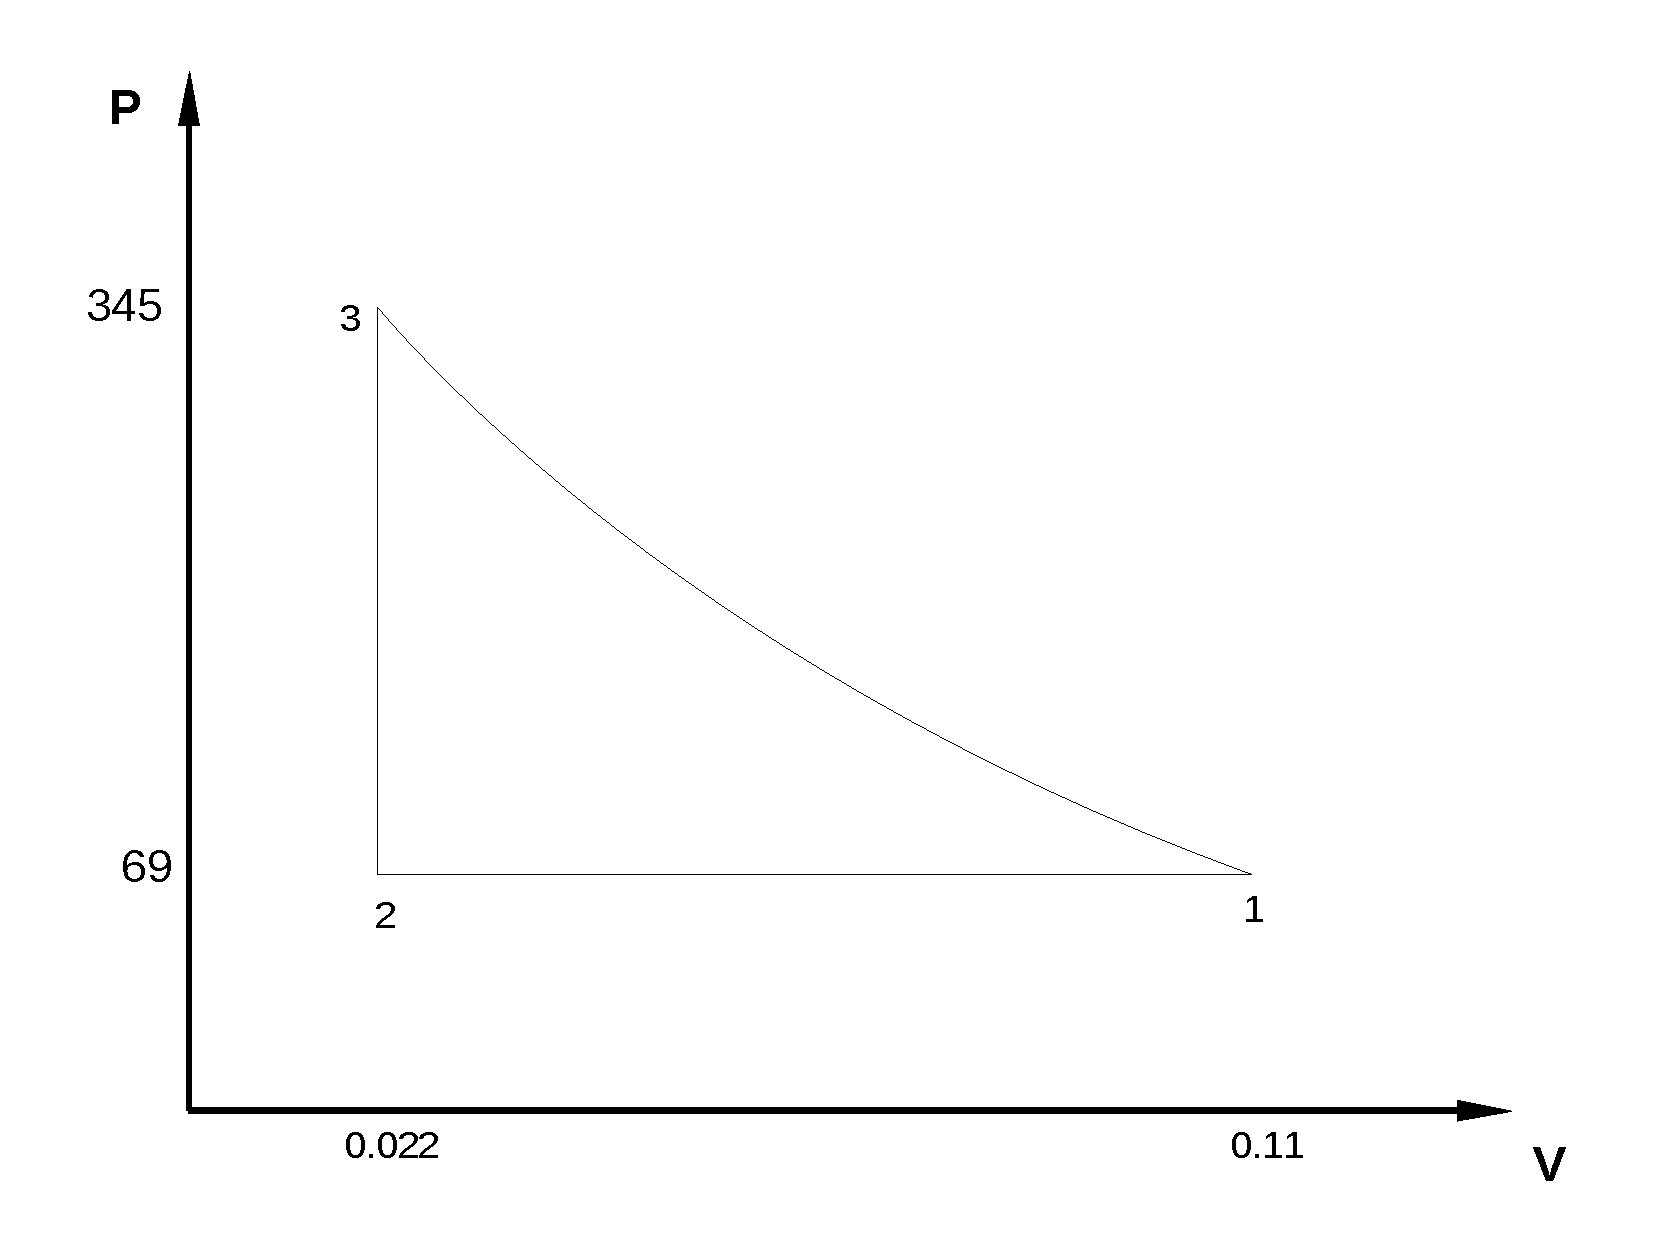
\includegraphics[width=10.cm,height=8.cm,clip]{./Pics/Exam_PV_Diagram}
\end{center}
}
\end{enumerate}

\end{enumerate}

%
\end{question}

\clearpage


%%%%%%%%%%%%%%%%%%%%%%%%%
%%% Question 03       %%%
%%%%%%%%%%%%%%%%%%%%%%%%%
\begin{question} 
\begin{enumerate}[(a)]
\item The energy conservation equation for a steady flow device with one inlet and one outlet can be written in the form:
\begin{align*}
 \dot{Q}-\dot{W}_{s} = \dot{m} \left(c_p T_\text{outlet} + \frac{u_{\text{outlet}}^2}{2}\right) - \dot{m} \left(c_p T_\text{inlet} + \frac{u_{\text{inlet}}^2}{2}\right).
\end{align*}
\begin{enumerate}[(i)]
\item Explain what the fluxes on the right-hand side of this equation represent. \marks{2}
\solution{$\dot{m} c_p T = \dot{m} h$ is a flux of enthalpy; \solmarks{1/2}

$\frac{1}{2} \dot{m} u^2$ is a flux of kinetic energy. \solmarks{1/2}}
\item What assumptions are required to derive this equation? \marks{4}
\solution{\begin{itemize}
\item The flow is steady and continuous;
\item The rate of heat addition and the rate of shaft work is are both constant;
\item The velocity and temperature profiles are uniform across the inlet and outlet cross section;
\item The change in gravitational energy is negligible;
\item No energy transfer due to viscous effects, electrodynamics, magnetism, surface tension, nuclear or chemical reactions.
\end{itemize}
One mark for each (up to four). \solmarks{4/4}}
\end{enumerate}

%%%%%%%%%%%%%%%%%%
\item The equation given above is valid for steady flow devices with one inlet and one outlet. Under the same modelling assumptions, state a modified version of this formula that is valid for steady flow devices with one inlet (whose properties are labelled 1) and two outlets (labelled 2 and 3). Give an equation that represents steady mass conservation in this case. \marks{4}
\solution{Energy conservation:
\begin{align*}
 \dot{Q}-\dot{W}_{s} = \dot{m}_2 \left(c_p T_2 + \frac{u_2^2}{2}\right) + \dot{m}_3 \left(c_p T_3 + \frac{u_3^2}{2}\right)- \dot{m}_1 \left(c_p T_1 + \frac{u_1^2}{2}\right).
\end{align*}\solmarks{3/4}

Mass conservation:
\begin{align*}
 \dot{m}_1 = \dot{m}_2 + \dot{m}_3.
\end{align*}\solmarks{1/4}
}

%%%%%%%%%%%%%%%%%%
\item Gas in a steady flow device with a circular inlet and two circular outlets does shaft work at a rate of $400$\,kW. The remaining known inlet and outlet properties are: 
\begin{center}
\begin{tabular}{|l |c |c |c |c |}
\hline
Property            & Inlet 1 & Outlet 2 & Outlet 3 & Units       \\
\hline
Diameter, $d$       & 0.05    & 0.2      & 0.5      & m$^{2}$     \\
Volume flux, $q$    & 1.8     & 0.5      & 20       & m$^{3}$/s   \\
Temperature, $T$    & 80      & 70       & 30       & $^{\circ}$C \\
Pressure, $p$       & 200     &          & 110      & kPa         \\
\hline 
\end{tabular}
\end{center}
If the gas behaves like an ideal gas with a gas specific gas constant $R=250$\,J/(kg.K) and specific heat capacity $c_{p}=1000$ J/(kg.K), then:
\begin{enumerate}[(i)]
\item Calculate the fluid velocity through each inlet and outlet; \marks{3}
\solution{The area of the inlet $A = \pi d^2/4$ and therefore
$A_1 = 7.853\times10^{-3}$\,m$^2$, $A_2 = 3.141\times10^{-2}$\,m$^2$ and $A_3 = 1.963\times10^{-1}$\,m$^2$. \solmarks{1/3}

The velocity through each inlet and outlet $u = q/A$. \solmarks{1/3}

Therefore $u_1=178.25$\,m/s, $u_2=50.930$\,m/s and $u_3=10.186$\,m/s.\solmarks{1/3}}

%%%%%%%%%%%%%%%%%%
\item Calculate the gas pressure at outlet 2; \marks{5}
\solution{The density at inlet 1 and outlet 3 are
\begin{align*}
 \rho_1 =& \frac{p_1}{R T_1} = \frac{400000}{250 \times (80 + 273.15)} = 4.5307\,\mbox{kg/m}^3, \\
 \rho_3 =& \frac{p_3}{R T_3} = \frac{120000}{250 \times (30 + 273.15)} = 1.5834\,\mbox{kg/m}^3.
\end{align*} \solmarks{1/5}

The mass flux at inlet 1 is $\dot{m}_1 = \rho_1 q_1 = 4.5307 \times 1.4 = 6.3429\,\mbox{kg/s}$, while the mass flux at outlet 2 is $\dot{m}_3 = \rho_3 q_3 = 1.5834 \times 2 = 3.1667\,\mbox{kg/s}$. \solmarks{1/5}

Mass conservation gives $\dot{m}_2 = \dot{m}_1 - \dot{m}_3 = 6.3429 - 3.1667 = 3.1762\,\mbox{kg/s}$.\solmarks{1/5}

The density at outlet 2 is $\rho_2 = \dot{m}_2/q_2 = 3.1762/1.6 = 1.9851\,\mbox{kg/m}^3$. \solmarks{1/5}

The pressure at outlet 2 is $p_2 = \rho_2 R T_2 = 1.9851 \times 250 \times (20 + 273.15) = 145500\,\mbox{Pa}$.\solmarks{1/5}
}

%%%%%%%%%%%%%%%%%%
\item Determine whether the steady flow device heats the gas or whether the gas heats the steady flow device. \marks{2}
\solution{Rearranging the energy equation
\begin{align*}
 \dot{Q} =& \dot{m}_2 \left(c_p T_2 + \frac{u_2^2}{2}\right) + \dot{m}_3 \left(c_p T_3 + \frac{u_3^2}{2}\right)- \dot{m}_1 \left(c_p T_1 + \frac{u_1^2}{2}\right) + \dot{W}_{s} \\
 =& (3.1762\times294400) + (3.1667\times303200) + (6.3429\times369000) + 400000 \\
 =& 960164.279690529 + 935211.868120291 - 2340770.89614347 + 400000 \\
 =& -45394\,\mbox{W}.
\end{align*}\solmarks{1/2}

The rate of heat addition to the gas is $-45$\,kW and therefore the gas gives off heat to the surroundings at a rate of $45$\,kW. \solmarks{1/2}
}
\end{enumerate}
\end{enumerate}
\end{question}

\clearpage


%%%%%%%%%%%%%%%%%%%%%%%%%
%%% Question 04       %%%
%%%%%%%%%%%%%%%%%%%%%%%%%
\begin{question} 
\begin{enumerate}[(a)]
\item A change in enthalpy $\d{h}$, entropy $\d{s}$ and pressure $\d{p}$ in an ideal gas are related through
\begin{align*}
 \d{h} = T \d{s} + V \d{p},
\end{align*}
where $T$ is the absolute temperature and $V$ is the specific volume.

Show that the change in entropy between the inlet and outlet of a compressor is given by
\begin{align*}
 s_\text{outlet} - s_\text{inlet} = c_p \ln \left(\frac{T_\text{outlet}}{T_\text{inlet}}\right) - R \ln \left(\frac{p_\text{outlet}}{p_\text{inlet}}\right).
\end{align*}
Here $c_p$ is the specific heat capacity at constant pressure and $R$ is the specific gas constant, which can both be assumed to be constant. \marks{6}
\solution{From the ideal gas equation
\begin{align*}
 V = \frac{R T}{p},
\end{align*}
while the gas specific enthalpy satisfies
\begin{align*}
 \d{h} = c_p \, \d{T}.
\end{align*}\solmarks{2/6}

If we eliminate the change in specific enthalpy $\d{h}$, the specific volume $V$ and rearrange, then
\begin{align*}
 \d{s} = c_p \frac{\d{T}}{T} - R \frac{\d{p}}{p}.
\end{align*} \solmarks{1/6}

Integrating from the inlet condition to the outlet condition
\begin{align*}
 \int_{s_\text{inlet}}^{s_\text{outlet}} \d{s} = \int_{T_\text{inlet}}^{T_\text{outlet}} c_p \frac{\d{T}}{T} - \int_{p_\text{inlet}}^{p_\text{outlet}} R \frac{\d{p}}{p}.
\end{align*} 
Assuming $c_p$ and $R$ are constant, then
\begin{align*}
 \left[s\right]_{s_\text{inlet}}^{s_\text{outlet}} = c_p \left[\ln T\right]_{T_\text{inlet}}^{T_\text{outlet}} - R \left[ \ln p \right]_{p_\text{inlet}}^{p_\text{outlet}},
\end{align*}
i.e.
\begin{align*}
 s_\text{outlet} - s_\text{inlet} = c_p \ln \left(\frac{T_\text{outlet}}{T_\text{inlet}}\right) - R \ln \left(\frac{p_\text{outlet}}{p_\text{inlet}}\right).
\end{align*} \solmarks{3/6}
}

%%%%%%%%%%%%%%%%%%
\item If the flow through the compressor is isentropic, then show that
\begin{align*}
 \frac{T_\text{outlet}}{T_\text{inlet}} = \left(\frac{p_\text{outlet}}{p_\text{inlet}}\right)^{1 - 1/\gamma},
\end{align*}
where $\gamma$ is the ratio of the specific heat capacities. \marks{4}
\solution{If the flow is isentropic, then $s_\text{outlet} - s_\text{inlet} = 0$ and
\begin{align*}
  \ln \left(\frac{T_\text{outlet}}{T_\text{inlet}}\right) = \frac{R}{c_p} \ln \left(\frac{p_\text{outlet}}{p_\text{inlet}}\right).
\end{align*} \solmarks{1/4}

By definition
\begin{align*}
 \frac{R}{c_p} = \frac{c_p - c_v}{c_p} = 1 - \frac{c_v}{c_p} = 1 - \frac{1}{\gamma}.
\end{align*}\solmarks{1/4}

Using properties of logarithms
\begin{align*}
  \ln \left(\frac{T_\text{outlet}}{T_\text{inlet}}\right) =  \ln \left[\left(\frac{p_\text{outlet}}{p_\text{inlet}}\right)^{1 - 1/\gamma}\right].
\end{align*} \solmarks{1/4}

Finally exponentiating both sides
\begin{align*}
 \frac{T_\text{outlet}}{T_\text{inlet}} =  \left(\frac{p_\text{outlet}}{p_\text{inlet}}\right)^{1 - 1/\gamma}.
\end{align*} \solmarks{1/4}
}

%%%%%%%%%%%%%%%%%%
\item An ideal gas with $R=260$\,J/(kg\,K) and $c_p=900$\,J/(kg\,K) flows through a well designed compressor in which the steady flow energy equation is given by
\begin{align*}
 \dot{W}_{s} = \dot{m} \left(h_\text{inlet} - h_\text{outlet}\right).
\end{align*}
The compressor is doing work on the gas at a rate of $500$\,kW, while the mass flux through the compressor is $4$\,kg/s. If the compressor has an inlet with pressure $p_\text{inlet}=100$\,kPa and temperature $T_\text{inlet}=25^\circ$C, and an outlet with pressure $p_\text{outlet}=350$\,kPa, then:
\begin{enumerate}[(i)]
\item Calculate the actual gas temperature at the outlet. \marks{3}
\solution{As $\d{h} = c_p \d{T}$, for the compressor
\begin{align*}
 \dot{W}_{s} = \dot{m} c_p \left(T_\text{inlet} - T_\text{outlet}\right),
\end{align*}
and hence 
\begin{align*}
 T_\text{outlet} = T_\text{inlet} - \frac{\dot{W}_{s}}{\dot{m} c_p} = (25 + 273.15) - \frac{-500000}{4 \times 900} = 437.04\,\mathrm{K} = 138.9^\circ\mathrm{C}.
\end{align*} \solmarks{3/3}
}

%%%%%%%%%%%%%%%%%%
\item Determine the isentropic efficiency of the compressor. \marks{7}
\solution{
The predicted gas temperature assuming isentropic compression is
\begin{align*}
 T_{\text{outlet,isentropic}} =& T_\text{inlet} \left(\frac{p_\text{outlet}}{p_\text{intlet}}\right)^{1 - 1/\gamma}.
\end{align*}\solmarks{1/7}

However, to use this formula we first must calculate the ratio of specific heats $\gamma$. The specific heat capacity at constant volume
\begin{align*}
 c_v = c_p - R = 900\,\mathrm{J/(kg\,K)} - 260\,\mathrm{J/(kg\,K)} = 640\,\mathrm{J/(kg\,K)}.
\end{align*}
Therefore
\begin{align*}
 \gamma = \frac{c_p}{c_v} = \frac{900\,\mathrm{J/(kg\,K)}}{640\,\mathrm{J/(kg\,K)}} = \frac{45}{32} = 1.4063.
\end{align*}\solmarks{1/7}

Now we can calculate the predicted isentropic compression temperature
\begin{align*}
 T_{\text{outlet,isentropic}} =& 298.15\,\mathrm{K} \times \left(\frac{350000\,\mathrm{Pa}}{100000\,\mathrm{Pa}}\right)^{13/45} = 428.164\,\mathrm{K}.
\end{align*}\solmarks{2/7}

The isentropic efficiency of the compressor
\begin{align*}
 \eta_s =& 100\% \times \left(\frac{T_{\text{outlet,isentropic}} - T_\text{inlet}}{T_{\text{outlet,actual}} - T_\text{inlet}}\right) \nonumber \\
=& 100\% \times \left(\frac{428.164 - 298.15}{437.039 - 298.15}\right) \nonumber \\
=& 100\% \times 0.936.
\end{align*}
Therefore the compressor has an isentropic efficiency of $94\%$. \solmarks{3/7}
}
\end{enumerate}
\end{enumerate}

\end{question}

\clearpage

%%%%%%%%%%%%%%%%%%%%%%%%%
%%% Question 05       %%%
%%%%%%%%%%%%%%%%%%%%%%%%%
\begin{question} 
An air stream with relative humidity $0.01$\,kg water/kg dry air passes through a duct at the rate of $1.2$\,kg\,s$^{-1}$. In the duct the air is first heated from $5^\circ$C to $20^\circ$C by heating coils and then humidified via the injection of hot steam. Air leaves the device at $25^\circ$C with a relative humidity of $60\%$. The air pressure is $101.325$\,kPa throughout.

\begin{enumerate}[(a)]
\item Determine the rate of heat addition in the heating section. \marks{5}
\solution{
In the simple heating section no water is added so $\omega_2 = \omega_1 = 0.01$\,kg water/kg dry air.

The enthalpies have contributions from dry air and water vapour with
\begin{align*}
 h_1 =& c_p T_1 + \omega_1 h_{g_1} = 1.005\times(5+273.15) + (0.01\times2510.1) = 304.64\,\mbox{kJ/kg} \\
 h_2 =& c_p T_2 + \omega_2 h_{g_2} = 1.005\times(20+273.15) + (0.01\times2537.4) = 320.00\,\mbox{kJ/kg}.
\end{align*}\solmarks{3/5}

Conservation of energy implies the rate of heat addition
\begin{align*}
 \dot{Q} = \dot{m}_a \left(h_2 - h_1\right) = 1.2\times(320.00 - 304.64) = 18.42\,\mbox{kJ/s}.
\end{align*}\solmarks{2/5}
}

%%%%%%%%%%%%%%%%%%
\item Determine the specific humidity of the air after the humidifying section. \marks{2}
\solution{From the psychrometric chart $\omega_3 = 0.012$\,kg water/kg dry air. \solmarks{2/2}}

%%%%%%%%%%%%%%%%%%
\item Determine the mass flow rate of steam required in the humidifying section. \marks{5}
\solution{Conservation of water vapour implies 
\begin{align*}
 \dot{m}_a \omega_2 + \dot{m}_w = \dot{m}_a \omega_3.
\end{align*} \solmarks{2/5}

Rearranging this expression the mass rate of steam required
\begin{align*}
 \dot{m}_w = \dot{m}_a \left(\omega_3 - \omega_2\right) = 1.2 \times (0.012 - 0.01) = 0.0024\,\mbox{kg/s}.
\end{align*}\solmarks{3/5}
}

%%%%%%%%%%%%%%%%%%
\item Explain why adding steam may be beneficial in this process. \marks{2}
\solution{As temperature increases the lower limit of the humidity range acceptable for human comfort also increases. Therefore if the temperature is increased and steam is not added (to increase the humidity), then the resulting air stream may have a humidity level that is uncomfortable for humans. \solmarks{3/3}}

%%%%%%%%%%%%%%%%%%
\item Sketch and identify the evolution of the different stages of this process on rough axes of a psychrometric chart. \marks{6}
\solution{
\begin{center}
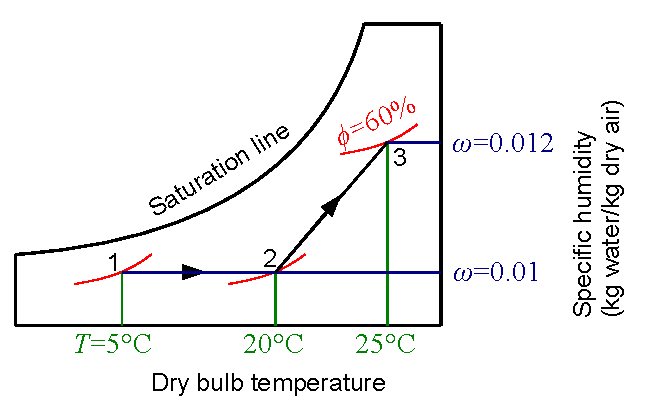
\includegraphics[width=0.7\textwidth]{./Pics/pChartHeatEx1}
\end{center}
Simple heating occurs between 1 and 2. Humidification occurs between 2 and 3. \solmarks{6/6}}
\end{enumerate}

You may assume that $c_p = 1005$\,J/(kg K), $R_a = 287$\,J/(kg K), while the enthalpy of saturated water vapour is $2510.1$\,kJ/kg at $5^\circ$C and $2537.4$\,kJ/kg at $20^\circ$C.
\end{question}


\vfill


\paperend

\begin{comment}
%\begin{landscape}
%\begin{center}
%\includegraphics[width=1.5\textwidth]{PsychrometricChart}
%\end{center}
{
  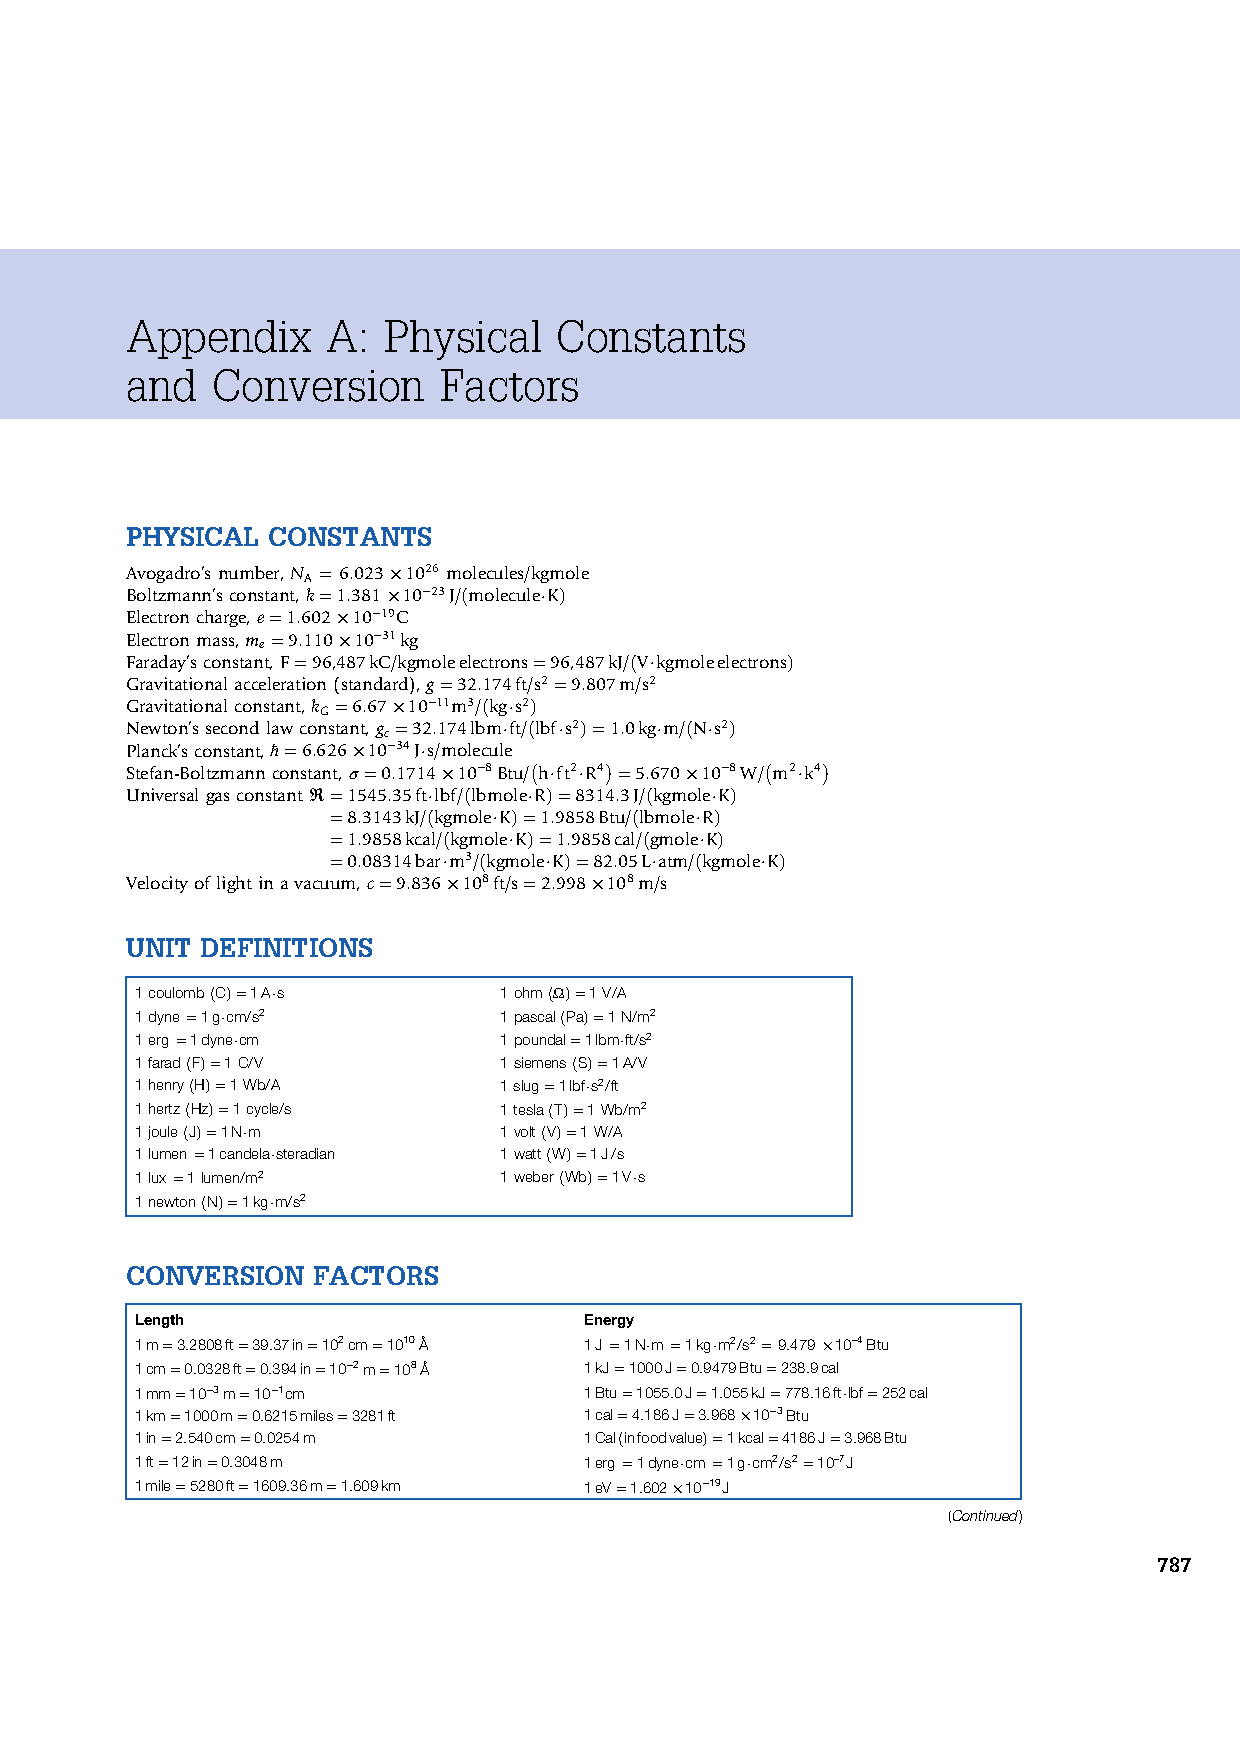
\includepdf[pages=-,fitpaper]{./Pics/UnitConversion}
  \includepdf[pages=-,fitpaper]{./Pics/PsychrometricChart}
  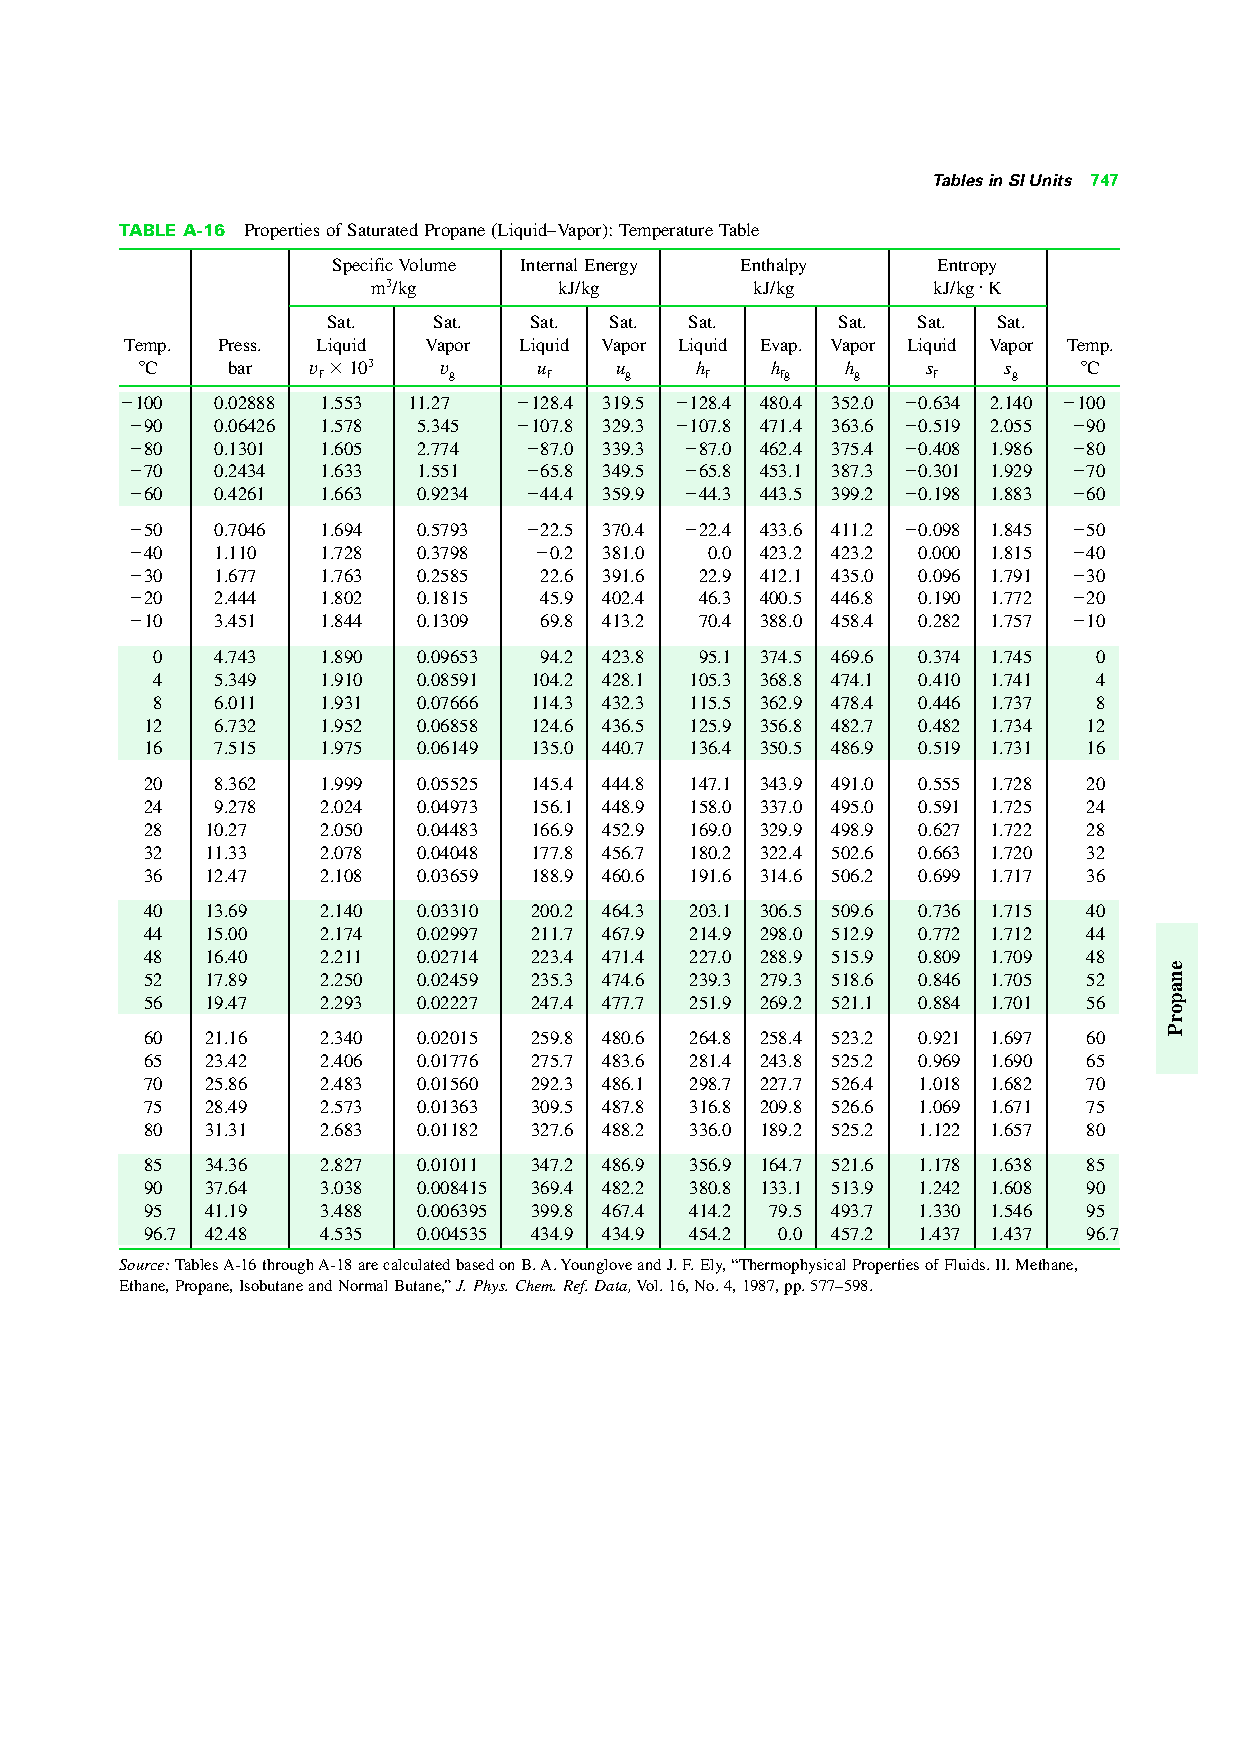
\includepdf[pages=-,fitpaper]{./Pics/nC3_Table}
%  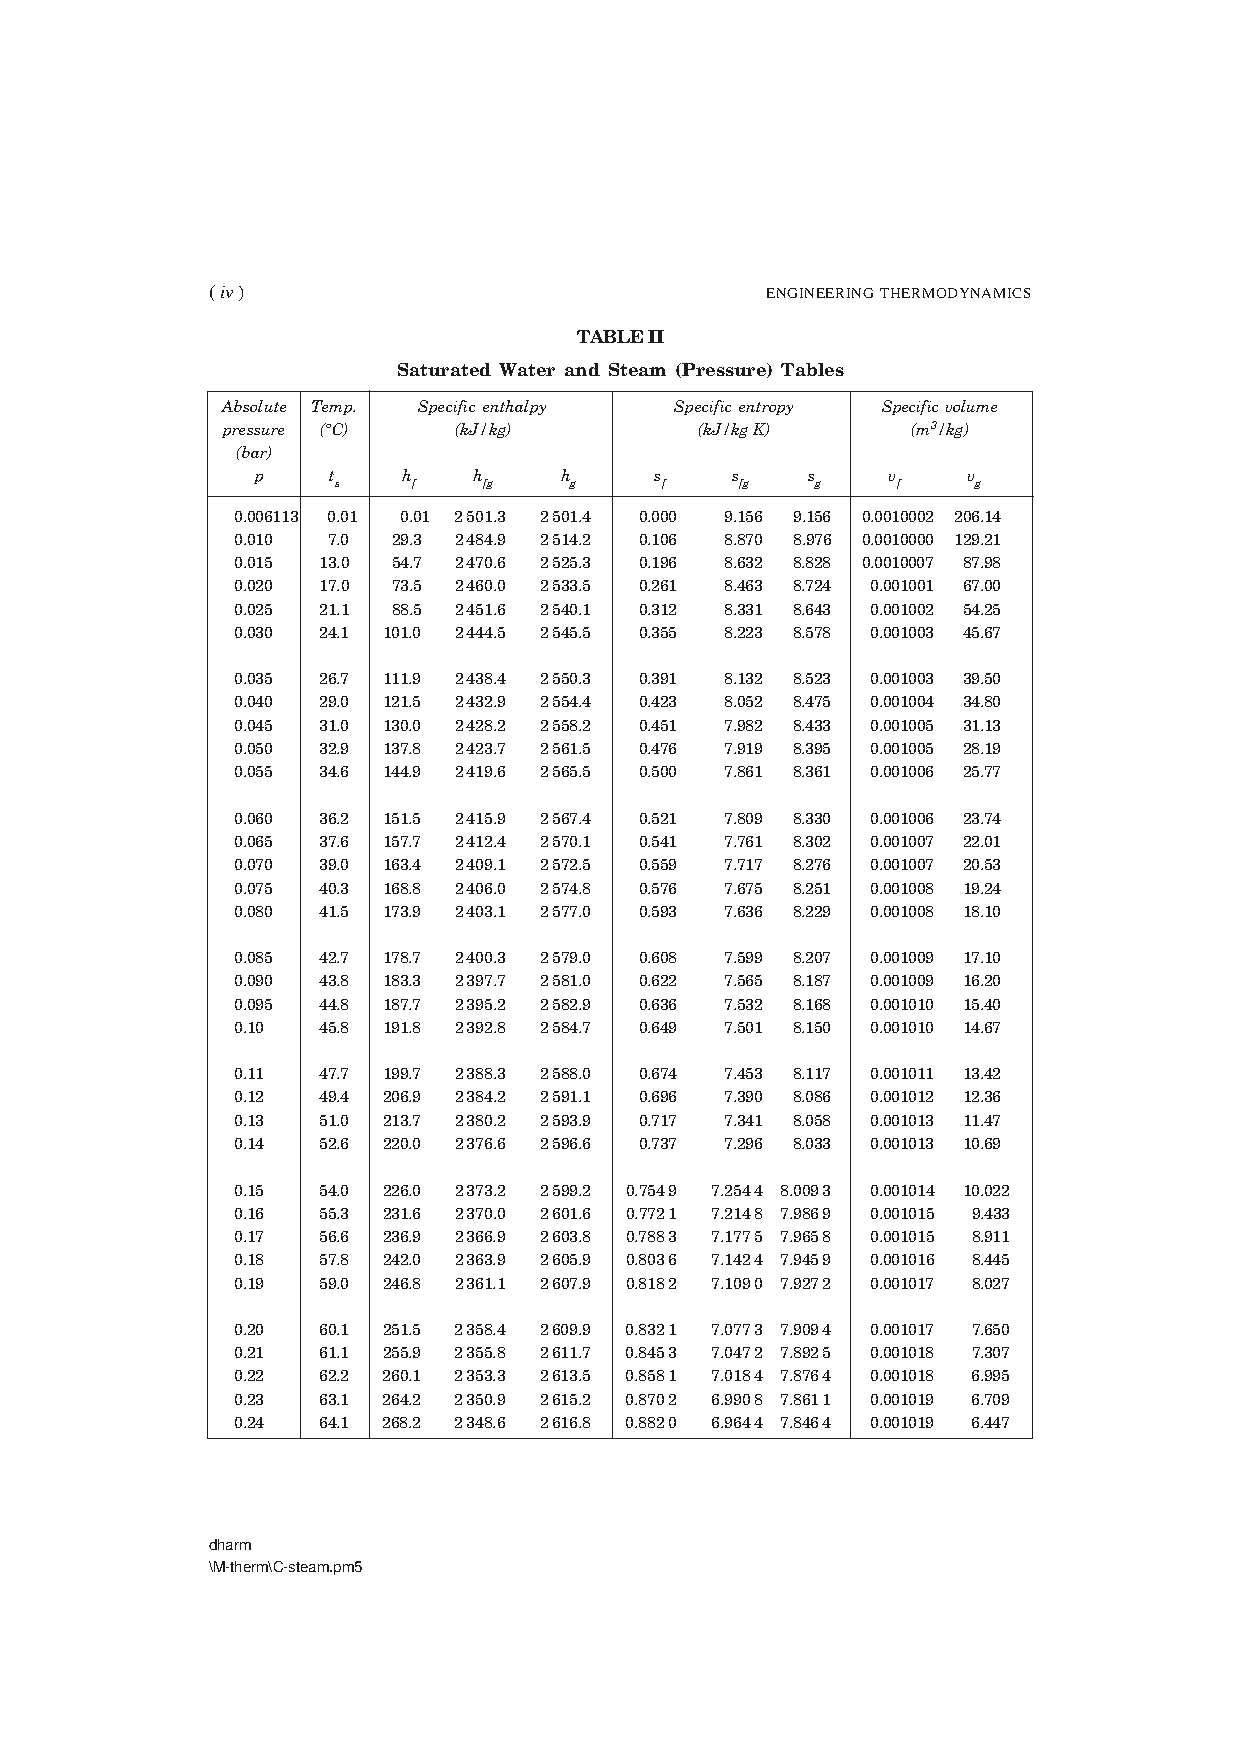
\includepdf[pages=-,fitpaper]{./Pics/SteamTable_2}
%  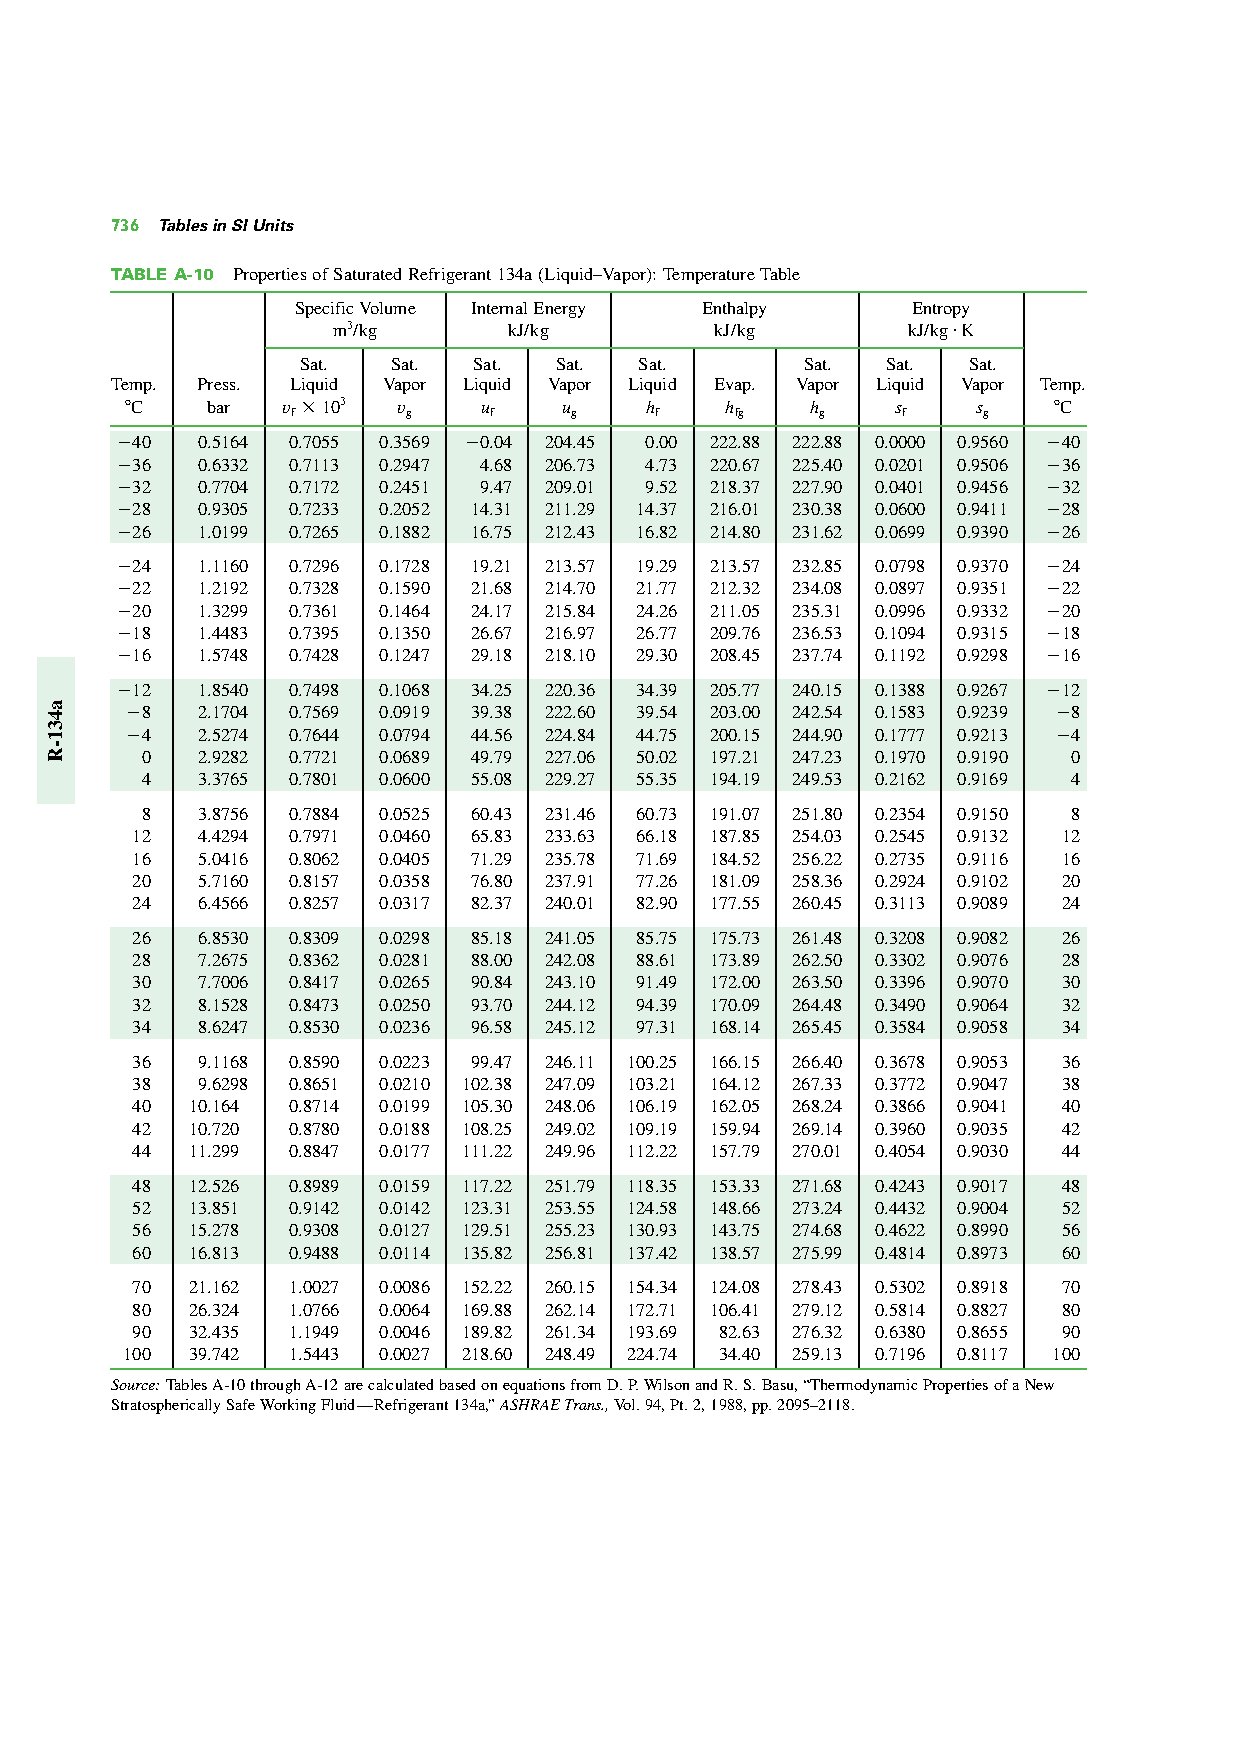
\includepdf[pages=-,fitpaper]{./Pics/Tables_R134}
}
%\end{landscape}
\end{comment}

\end{document}
